\documentclass[manuscript, screen, review]{acmart}
\usepackage{tikz}
\usepackage{pgfplots}
\pgfplotsset{compat=1.18}

\usetikzlibrary{positioning}
\setcopyright{acmcopyright}
\copyrightyear{2026}
\acmYear{2026}
\acmDOI{XXXXXXX.XXXXXXX}

\begin{document}

\title{An Explainable AI Decision Layer for Human-in-the-loop SAP ERP Workflow Integration in Supply Chain Operations}

\author{Majd Kassem}
\affiliation{
  \institution{Department of Electronics Technology, Faculty of Electrical Engineering and Informatics, Budapest University of Technology and Economics}
  \streetaddress{Műegyetem rkp. 3.}
  \city{Budapest}
  \postcode{H-1111}
  \country{Hungary}
}
\email{mjdwassouf@gmail.com}

\author{Engida Ephrem Alamerew}
\affiliation{
  \institution{Department of Electronics Technology, Faculty of Electrical Engineering and Informatics, Budapest University of Technology and Economics}
  \streetaddress{Műegyetem rkp. 3.}
  \city{Budapest}
  \postcode{H-1111}
  \country{Hungary}
}
\email{ephremalamerewengida@edu.bme.hu}

\author{Villányi Balázs János}
\affiliation{
  \institution{Department of Electronics Technology, Faculty of Electrical Engineering and Informatics, Budapest University of Technology and Economics}
  \streetaddress{Műegyetem rkp. 3.}
  \city{Budapest}
  \postcode{H-1111}
  \country{Hungary}
}
\email{villanyi.balazs@vik.bme.hu}


\renewcommand{\shortauthors}{Surname, et al.}

\begin{abstract}
Traditional statistical process control and enterprise systems are predominantly retrospective, limiting proactive operational intervention. This study presents an SAP-oriented predictive decision framework that integrates logistics transaction data, supervised machine learning, probabilistic risk estimation, human-in-the-loop decision control, SAP-oriented workflow simulation, and cost-sensitive economic evaluation. Using 180,519 logistics observations from the DataCo Supply Chain dataset, the framework evaluates Logistic Regression, CART, Random Forest, XGBoost, and LightGBM models. Random Forest achieved the highest cross-validated ROC-AUC performance, while calibrated prediction probabilities were transformed into operational risk levels to support decision-making. The proposed decision layer converts predictive outputs into interpretable risk states, recommended actions, human review processes, workflow execution, and economic evaluation. Experimental results demonstrate that integrating predictive analytics with SAP-oriented decision processes can improve operational intervention capability and provide measurable business value. The study highlights the importance of bridging machine learning predictions with explainable and human-centered enterprise decision workflows.
\end{abstract}

\keywords{SAP ERP, Data Integration, Explainable Artificial Intelligence, Human-in-the-Loop Decision Making, Predictive Analytics, Machine Learning, Operational Optimization, Enterprise Systems}

\maketitle

\section{Introduction}

\subsection{Research Background}

Enterprise Resource Planning (ERP) systems remain central to managing business processes, 
resource planning, and operational execution in supply chain environments. 
SAP-based platforms are widely used to coordinate these activities across enterprise 
functions \cite{monk2006sap}.
At the same time, logistics and supply chain operations generate large volumes of 
transactional and operational data that can be used for predictive analysis and 
decision support \cite{constante2019dataco}.
Machine-learning methods provide opportunities to 
extract predictive information from such data and support 
more proactive operational decisions
 \cite{xu2021industry40,olan2024xai_supplychain}.
However, integrating predictive analytics into 
enterprise workflows involves challenges beyond model accuracy, 
including interoperability, interpretability, 
decision transparency, and the appropriate involvement 
of human decision-makers \cite{amershi2019guidelines,li2024xai_supplychain}.

\subsection{Related Research}

Recent reviews of explainable AI (XAI) in decision-support systems
identify interpretability, transparency, trust, and the integration of
explanations into decision processes as recurring research themes
\cite{kostopoulos2024xai_dss,ezeji2024explainable_dss,fanfani2026human_dss}.
In supply-chain applications, XAI has mainly been used to make
predictive models easier to understand and to provide decision-makers
with additional information about model outputs
\cite{olan2024xai_supplychain,kosasih2024xai_supplychain}.

A particularly relevant study by Reis et al. investigated a
context-aware approach for selecting XAI methods according to the
requirements of business stakeholders. The study included human
participants and used supply-chain demand data to evaluate the
approach \cite{reis2025contextxai}. This is relevant to the present
work because it treats explainability as part of a decision-support
setting rather than only as a property of an individual prediction
model.

However, the focus of this line of research remains primarily on
model explanation, stakeholder requirements, and decision support.
It does not directly address the complete operational path from a
predictive output to a predefined enterprise action, followed by
human review when required. Similarly, the reviewed supply-chain XAI
studies do not establish a specific workflow mechanism that connects
risk classifications produced by a predictive model to SAP-oriented
enterprise actions.

The gap considered in this study is therefore operational rather than
algorithmic. The study does not propose a new XAI algorithm. Instead,
it examines how predictive outputs can be organized into risk states,
mapped to workflow actions, and selectively escalated to human
review within an SAP-oriented supply-chain process.
\subsection{Research Gap and Problem Statement}

The reviewed studies show that predictive analytics, XAI, and human-centered decision support have each been investigated in supply-chain and enterprise contexts. However, these studies generally focus on individual stages of the decision process, such as prediction, model explanation, stakeholder requirements, or human interaction \cite{kostopoulos2024xai_dss,fanfani2026human_dss,olan2024xai_supplychain,kosasih2024xai_supplychain,reis2025contextxai}.

What remains less clearly addressed is the operational connection between these stages. In particular, a predictive result must be converted into an interpretable operational state, mapped to an appropriate enterprise action, and escalated to a human decision-maker when the case requires additional judgment. Human-AI interaction research emphasizes maintaining human understanding and control in such processes \cite{amershi2019guidelines}.

This study therefore focuses on a narrower operational gap: the organization of prediction, risk assessment, workflow action, and selective human review as one decision layer within an SAP-oriented supply-chain process. The contribution is consequently not a new prediction or XAI algorithm, but the integration of these existing capabilities into an explicit workflow-oriented decision process.

The research problem is formulated as follows:

\begin{quote}
How can logistics and supply-chain predictions be transformed into explainable risk-based decisions, connected to SAP-oriented workflow actions, and selectively escalated for human review?
\end{quote}

\subsection{Research Objectives}

The objectives of this study are:

\begin{enumerate}
\item Assess the predictive performance of machine-learning models for logistics and supply-chain risk prediction.
\item Examine whether transforming predictions into risk-based states provides more useful operational decision support.
\item Evaluate how workflow mapping can translate risk states into predefined SAP-oriented actions.
\item Assess the role of human review in controlling higher-risk or uncertain cases.
\item Evaluate the overall framework in terms of predictive performance, operational effectiveness, and human-review requirements.
\end{enumerate}


\subsection{Research Contribution}

This paper presents a workflow-oriented decision layer that uses
logistics and supply-chain data to produce risk estimates and map them
to predefined operational actions.

The contribution lies in combining predictive modelling, risk
classification, human review, workflow simulation, and decision
evaluation in a single SAP-oriented process, rather than proposing a
new machine-learning or XAI algorithm.

\section{Methodology}

\subsection{Overall Framework}

The methodology follows a sequence of steps that starts with logistics
data preparation and predictive modelling and then examines how model
outputs can be used in an operational decision process. The study
combines exploratory data analysis, supervised machine learning,
probability calibration, risk classification, human review simulation,
SAP-oriented workflow simulation, and cost-sensitive evaluation.

The framework consists of the following stages:
\begin{enumerate}
    \item data preparation and exploratory analysis;
    \item predictive model development and comparison;
    \item model diagnostics and performance analysis;
    \item construction of operational risk levels;
    \item probability calibration;
    \item cost-sensitive decision evaluation;
    \item human-in-the-loop decision simulation;
    \item SAP-oriented workflow simulation;
    \item economic evaluation and sensitivity analysis.
\end{enumerate}

The sequence of the decision-layer process is shown in
Fig.~\ref{fig:decision_pipeline}. The figure represents the workflow
implemented in the study, rather than a deployed SAP system.

\begin{figure}[htbp]
\centering
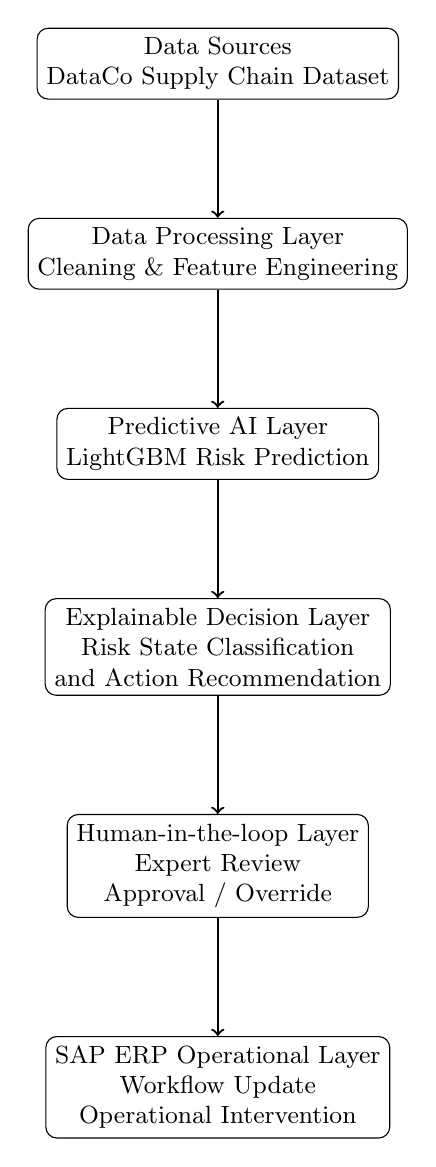
\begin{tikzpicture}[
node distance=1.5cm,
every node/.style={
    draw,
    rounded corners,
    align=center,
    minimum width=3.2cm,
    minimum height=0.9cm,
    font=\small
},
arrow/.style={->, thick}
]

\node (data) {
Data Sources\\
DataCo Supply Chain Dataset
};

\node (process) [below=of data] {
Data Processing Layer\\
Cleaning \& Feature Engineering
};

\node (ai) [below=of process] {
Predictive AI Layer\\
LightGBM Risk Prediction
};

\node (decision) [below=of ai] {
Explainable Decision Layer\\
Risk State Classification\\
and Action Recommendation
};

\node (human) [below=of decision] {
Human-in-the-loop Layer\\
Expert Review\\
Approval / Override
};

\node (sap) [below=of human] {
SAP ERP Operational Layer\\
Workflow Update\\
Operational Intervention
};

\draw[arrow] (data) -- (process);
\draw[arrow] (process) -- (ai);
\draw[arrow] (ai) -- (decision);
\draw[arrow] (decision) -- (human);
\draw[arrow] (human) -- (sap);

\end{tikzpicture}
\caption{Decision-layer process used in the study, from prediction to
risk assessment, operational action, and human review.}
\Description{Decision-layer workflow from prediction through risk assessment, operational action, and human review.}
\label{fig:decision_pipeline}
\end{figure}

The predictive models estimate the probability of late delivery. These
probabilities are then converted into operational risk levels and used
to assign predefined actions. Cases meeting the specified review
conditions are passed to a simulated human-review step. The resulting
process is evaluated using predictive, operational, and economic
measures.

The SAP component is treated as a workflow-oriented representation of
how the resulting decisions could be connected to enterprise
processes. It does not represent a live SAP implementation or direct
execution of SAP transactions.

The architecture used to represent this relationship is shown in
Fig.~\ref{fig:sap_architecture}.
\begin{figure}[htbp]
\centering
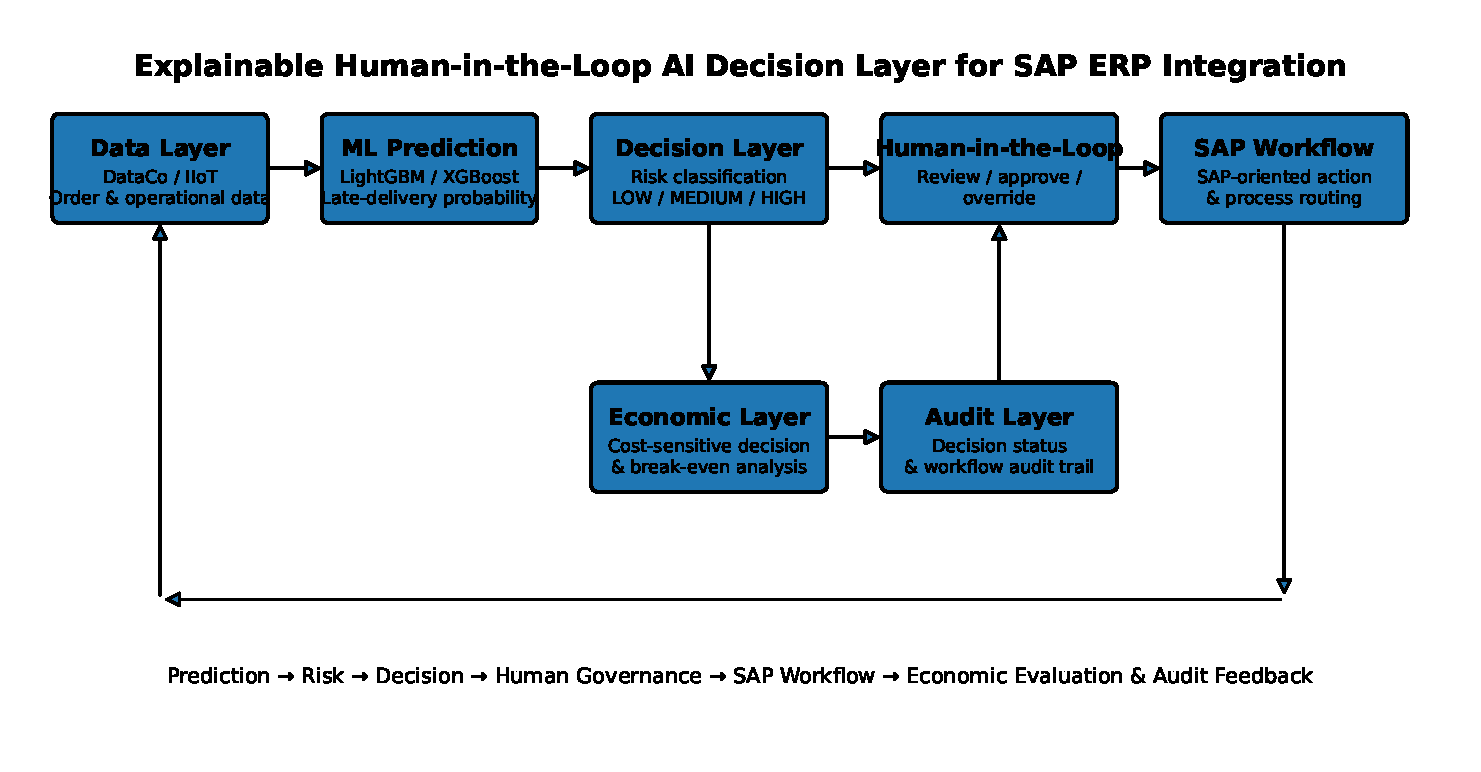
\includegraphics[width=\columnwidth]{../../results/sap_architecture_diagram.pdf}
\caption{SAP-oriented decision-layer architecture.}
\Description{SAP-oriented architecture connecting the AI decision layer with enterprise workflow processes.}
\label{fig:sap_architecture}
\end{figure}

\subsection{Data Preparation and Process Analysis}

The empirical evaluation uses the DataCo SMART SUPPLY CHAIN FOR BIG DATA
ANALYSIS dataset, originally released through Mendeley Data
\cite{constante2019dataco}. The dataset contains 180,519 order-level
observations. The prediction target is the binary variable \\
\texttt{Late\_delivery\_risk}, which indicates whether an order is
classified as being at risk of late delivery.

The analysis considers operational variables related to shipping mode,
market, customer segment, order region, order-item quantity, product
price, and other logistics attributes available in the dataset.

The raw data are processed before model training to obtain a consistent
feature representation. Categorical variables are encoded into
machine-learning-compatible representations, while numerical variables
are preserved unless a specific modelling procedure requires further
transformation. Variables that directly reveal the target or are
available only after the outcome are excluded to reduce target leakage.

The resulting feature matrix is represented as

\begin{equation}
X \in \mathbb{R}^{n \times p},
\end{equation}

where $n$ denotes the number of observations and $p$ denotes the number
of predictive features. The corresponding target vector is

\begin{equation}
y \in \{0,1\}^{n}.
\end{equation}

The same processed observations are then used for the subsequent
predictive modelling and decision-layer evaluation, with the specific
train--test procedure described in the following subsection.
\subsection{Process Capability Baseline}

Process capability analysis is used as a statistical baseline to
describe the historical performance of the selected logistics process.
Let $X$ denote the quality characteristic, with process mean $\mu$,
standard deviation $\sigma$, and specification limits $LSL$ and $USL$.
The capability index $C_{pk}$ is defined as
\cite{montgomery2019introduction}:

\begin{equation}
C_{pk} =
\min\left(
\frac{USL-\mu}{3\sigma},
\frac{\mu-LSL}{3\sigma}
\right).
\end{equation}

In this study, $C_{pk}$ is used only as a descriptive baseline for
historical process capability. A value below $1.33$ is interpreted using
the commonly applied capability criterion
\cite{montgomery2019introduction}.

The capability analysis is not used to generate the prediction target
or to replace the machine-learning models. Instead, it provides a
process-level reference against which the subsequent transaction-level
risk analysis can be interpreted.

\subsection{Predictive Model Development}

Five supervised learning models are evaluated for late-delivery risk:
Logistic Regression, Classification and Regression Trees (CART)
\cite{breiman1984classification}, Random Forest
\cite{breiman2001random}, XGBoost \cite{chen2016xgboost}, and LightGBM
\cite{ke2017lightgbm}.

For each observation $i$, the models estimate the probability of a
late-delivery event:

\begin{equation}
\hat{p}_i = P(Y_i=1\mid X_i),
\label{eq:prediction_probability}
\end{equation}

where $\hat{p}_i$ is the predicted probability and $X_i$ is the
corresponding feature vector.

Model performance is compared using cross-validation. ROC-AUC is used
as the primary discrimination measure because it evaluates the ability
of a classifier to distinguish positive from negative observations
across decision thresholds \cite{fawcett2006introduction}.

CART is also retained as an interpretable baseline because its tree
structure provides explicit decision rules. Its node impurity is
measured using the Gini index \cite{breiman1984classification}:

\begin{equation}
I(t)=1-\sum_{k=1}^{C}p_k^2,
\end{equation}

where $p_k$ denotes the proportion of observations belonging to class
$k$ at node $t$.

The resulting model probabilities are subsequently used as inputs to
risk classification and the decision-layer analysis.

\subsection{Probability Calibration}

Because the decision layer uses predicted probabilities to define risk
levels, calibration is evaluated in addition to discrimination
\cite{niculescu2005predicting,guo2017calibration}.

The Brier Score measures the accuracy of probabilistic predictions
\cite{brier1950verification}:

\begin{equation}
BS=\frac{1}{N}\sum_{i=1}^{N}(\hat{p}_i-y_i)^2.
\end{equation}

Expected Calibration Error (ECE) is also calculated by grouping
predictions into $B$ probability bins
\cite{naeini2015obtaining,guo2017calibration}:

\begin{equation}
ECE=
\sum_{b=1}^{B}
\frac{|S_b|}{N}
\left|
\operatorname{acc}(S_b)
-
\operatorname{conf}(S_b)
\right|.
\end{equation}

Here, $S_b$ denotes the observations assigned to bin $b$.

These measures are used to determine whether predicted probabilities
provide a sufficiently reliable basis for the subsequent risk
classification and decision thresholds.

\subsection{Cost-Sensitive Decision Evaluation}

Predictive performance alone does not determine whether an operational
intervention is preferable. The decision layer therefore evaluates
alternative actions using assumed costs for late delivery and
intervention. This follows the cost-sensitive decision perspective,
where the consequences of classification errors are incorporated into
the decision process \cite{elkan2001foundations}.

For observation $i$, the expected cost of taking no intervention is
defined as:

\begin{equation}
C_{\mathrm{no\ intervention},i}
=
\hat{p}_i C_L,
\label{eq:baseline_cost}
\end{equation}

where $\hat{p}_i$ is the predicted probability of late delivery and
$C_L$ is the assumed cost associated with a late-delivery event.

For an intervention decision, the expected cost is represented as:

\begin{equation}
C_{\mathrm{intervention},i}
=
C_{\mathrm{residual},i}
+
I_i C_I,
\label{eq:decision_cost}
\end{equation}

where $C_{\mathrm{residual},i}$ represents the estimated remaining
late-delivery cost after intervention, $C_I$ is the assumed intervention
cost, and $I_i\in\{0,1\}$ indicates whether the intervention is applied.

The difference between the two alternatives is expressed as:

\begin{equation}
S =
C_{\mathrm{no\ intervention}}
-
C_{\mathrm{intervention}}.
\label{eq:saving}
\end{equation}

A positive value indicates that the intervention has a lower estimated
cost under the specified assumptions. The corresponding relative
difference is:

\begin{equation}
SR =
\frac{S}{C_{\mathrm{no\ intervention}}}.
\end{equation}

These results are interpreted as scenario-based economic estimates,
since the dataset does not provide directly observed intervention
costs or verified financial savings. Sensitivity analysis is therefore
used to examine how changes in the assumed cost parameters affect the
preferred decision.

\subsection{Cost Sensitivity and Break-Even Analysis}

The economic evaluation depends on assumed costs for late delivery and
operational intervention. A sensitivity analysis is therefore performed
to examine how changes in these assumptions affect the preferred
decision. This follows the cost-sensitive decision perspective, where
the consequences of alternative decisions are considered alongside
classification performance \cite{elkan2001foundations}.

For each scenario, intervention is considered preferable when:

\begin{equation}
C_{\mathrm{decision}} <
C_{\mathrm{baseline}}.
\end{equation}

For a given observation, the break-even intervention cost is the
difference between the expected cost without intervention and the
estimated residual cost after intervention:

\begin{equation}
C_{I,\mathrm{BE}}
=
C_{\mathrm{baseline}}
-
C_{\mathrm{residual}}.
\label{eq:break_even_cost}
\end{equation}

An intervention is economically preferable when:

\begin{equation}
C_I < C_{I,\mathrm{BE}}.
\end{equation}

The analysis is used to identify how sensitive the resulting decisions
are to the assumed cost parameters. Since the dataset does not contain
verified intervention costs, the results are interpreted as scenario
estimates rather than measured financial savings.

\begin{figure}[htbp]
\centering
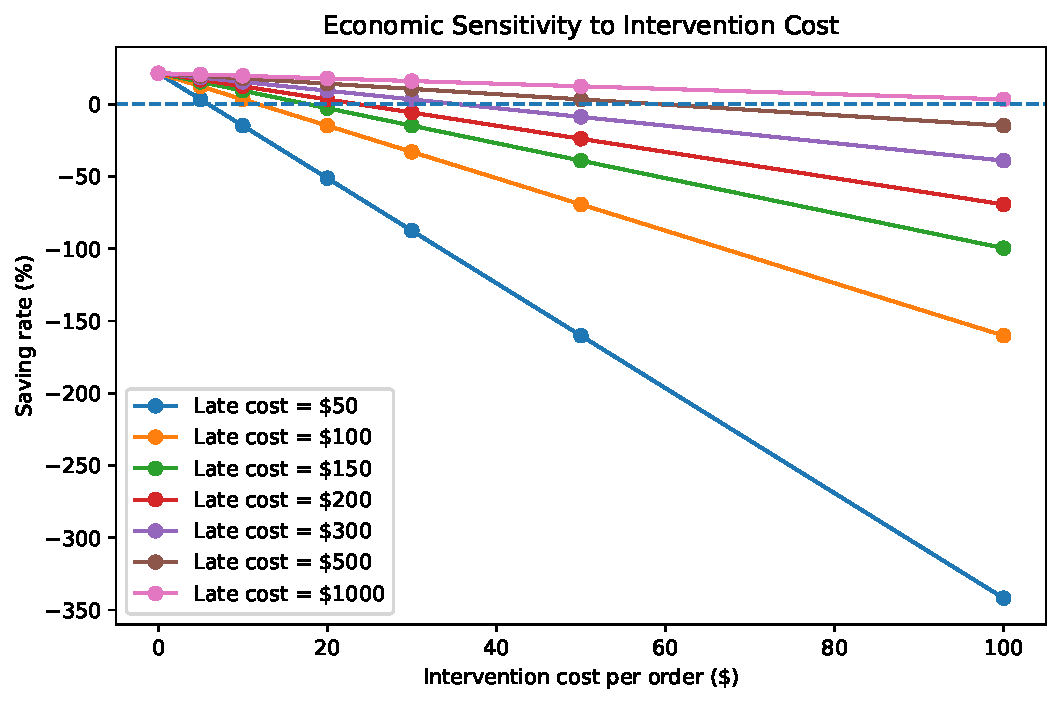
\includegraphics[width=0.85\linewidth]{../../results/cost_sensitivity.pdf}
\caption{Sensitivity of the estimated intervention benefit to assumed
late-delivery and intervention costs.}
\Description{Sensitivity analysis showing how assumed late-delivery and
intervention costs affect the estimated economic benefit of intervention.}
\label{fig:cost_sensitivity}
\end{figure}


\subsection{Human-in-the-Loop Decision Process}

Human review is introduced as a selective control step for cases
identified by the decision rules as requiring additional assessment.
This follows human-AI interaction principles that emphasize user
understanding, control, and the ability to intervene in AI-supported
decisions \cite{amershi2019guidelines,shneiderman2020human}.

The evaluated decision flow is:

\begin{equation}
\begin{aligned}
\mathrm{Prediction}
&\rightarrow \mathrm{Risk\ Assessment}\\
&\rightarrow \mathrm{Action\ Selection}\\
&\rightarrow \mathrm{Human\ Review\ (if\ required)}\\
&\rightarrow \mathrm{Final\ Decision}.
\end{aligned}
\end{equation}

LOW-risk observations follow the standard processing path. MEDIUM- and
HIGH-risk observations are eligible for human review according to the
predefined decision rules. Human review is simulated in the prototype
and does not represent interaction with actual SAP users.

The analysis records the number and proportion of observations
escalated for review. These measures are used to estimate the review
workload associated with the decision policy and to assess whether the
policy limits human intervention to selected cases.

\subsection{SAP-Oriented Workflow Integration}

The resulting decisions are represented as an SAP-oriented workflow to
examine how predictive outputs can be incorporated into an enterprise
decision process. This representation is a workflow simulation and
does not execute SAP transactions.

The simulated workflow consists of five logical stages:

\begin{enumerate}
\item logistics and operational data;
\item machine-learning prediction;
\item risk assessment and decision rules;
\item human-review control;
\item SAP-oriented workflow action.
\end{enumerate}

For each observation, the decision layer produces a structured record
containing the predicted late-delivery probability, assigned risk
category, selected action, workflow state, human-review requirement,
and final decision status.

This representation makes the transition from a probabilistic model
output to an operational decision explicit. It also records the main
elements of the decision path, allowing the selected action and any
human intervention to be traced back to the corresponding prediction
and decision rule. Traceability and human control are relevant
considerations in AI-supported decision processes
\cite{amershi2019guidelines,shneiderman2020human}.

A lightweight Streamlit prototype is used to simulate the workflow.
The prototype accepts the selected operational attributes, generates
the calibrated risk probability, applies the predefined decision
rules, and displays the resulting workflow action and human-review
status. The estimated economic effect of the selected decision is also
reported.

The prototype is used for evaluation and demonstration of the
decision process. It is not considered a production SAP integration,
and it does not establish a connection to or execute transactions in
an SAP system.

\subsection{End-to-End Evaluation}

The complete framework is evaluated using representative cases from
the three operational risk categories: LOW, MEDIUM, and HIGH. The
evaluation considers the complete decision path rather than predictive
performance alone, linking the model output to the resulting risk
classification, selected action, human-review status, workflow state,
and estimated cost.

For each evaluated observation, the decision record is represented as:

\begin{equation}
D_i =
\left\{
\hat{p}_i,
R_i,
A_i,
H_i,
W_i,
F_i,
C_{\mathrm{baseline},i},
C_{\mathrm{decision},i}
\right\},
\label{eq:decision_record}
\end{equation}

where $\hat{p}_i$ is the predicted late-delivery probability, $R_i$
is the assigned risk category, $A_i$ is the selected operational
action, $H_i$ indicates whether human review is required, $W_i$
represents the workflow state, and $F_i$ records the final decision
status.

The end-to-end evaluation checks whether these elements remain
consistent with the predefined decision rules. It also examines the
number of cases requiring human review and the estimated economic
effect of the resulting decisions.

This stage therefore evaluates the proposed decision layer as a
complete process, from probabilistic prediction to operational
decision, rather than treating model accuracy as the final evaluation
criterion.

\section{Results and Discussion}
The results are presented in the same sequence as the evaluation
procedure described in the methodology. The analysis first establishes
the characteristics of the dataset and historical delivery outcomes,
then evaluates predictive performance and probability calibration.
The subsequent results examine risk stratification, cost-sensitive
decisions, human-review workload, and the simulated SAP-oriented
workflow. This structure separates model performance from the
operational and economic evaluation of the resulting decisions.
\subsection{Baseline Statistical Assessment}

The analysis was performed on 180,519 order-level observations from the
DataCo Supply Chain dataset \cite{constante2019dataco}. The dataset
contains operational attributes related to shipping, markets, order
regions, product characteristics, and delivery performance.

The target variable, \texttt{Late\_delivery\_risk}, was treated as a
binary outcome representing whether an order was associated with a
late-delivery event.

Before predictive modelling, a baseline statistical assessment was
conducted to characterize the historical data distribution and identify
initial relationships between operational attributes and delivery
outcomes. These analyses describe the dataset characteristics and do
not represent predictive performance.

The distribution of the target variable is summarized in
Table~\ref{tab:target_distribution}.

\begin{table}[htbp]
\caption{Distribution of late-delivery risk classes.}
\Description{Table showing the distribution of late-delivery risk classes within the dataset, indicating the number of observations for each class category.}
\label{tab:target_distribution}
\centering
\begin{tabular}{rrr}
\toprule
Class & Count & Percentage \\
\midrule
1 & 98977 & 54.830000 \\
0 & 81542 & 45.170000 \\
\bottomrule
\end{tabular}

\end{table}

The target distribution provides an indication of the proportion of
late and non-late delivery cases. This information is considered during
later model evaluation because class imbalance may influence
classification metrics.

Categorical associations between operational attributes and the target
variable were then examined using contingency analysis and chi-square
testing.

The results of these tests are presented in
Table~\ref{tab:chi_square}.

\begin{table}[htbp]
\caption{Chi-square analysis of categorical operational attributes.}
\Description{Table presenting the results of the chi-square analysis for categorical operational attributes, showing statistical association metrics with the late-delivery risk outcome.}
\label{tab:chi_square}
\centering
\begin{tabular}{lrrr}
\toprule
Feature & Chi\_square & p\_value & Degrees\_of\_freedom \\
\midrule
Shipping Mode & 37716.042505 & 0.000000 & 3 \\
Market & 8.650714 & 0.070448 & 4 \\
Customer Segment & 1.024740 & 0.599074 & 2 \\
Order Region & 74.933614 & 0.000000 & 22 \\
Department Name & 6.666695 & 0.756492 & 10 \\
Category Name & 42.889228 & 0.717981 & 49 \\
\bottomrule
\end{tabular}

\end{table}

The chi-square analysis identifies operational attributes that show
different historical late-delivery patterns. These observations are
used as descriptive evidence for feature analysis and do not imply
causal relationships. Predictive relationships are evaluated separately
through the machine-learning models presented in the following section.

\subsection{Predictive Model Performance}

Five supervised learning models were evaluated for late-delivery risk
prediction: Logistic Regression, CART, Random Forest, XGBoost, and
LightGBM \cite{breiman1984classification,breiman2001random,chen2016xgboost,ke2017lightgbm}.
The models were compared using mean cross-validated ROC-AUC as the
primary discrimination metric. ROC-AUC was selected because it measures
the ability of a classifier to rank positive cases higher than negative
cases across different classification thresholds \cite{fawcett2006introduction}.

The comparative results are presented in Table~\ref{tab:model_performance}.

\begin{table}[htbp]
\centering
\caption{Predictive Model Performance}
\Description{Table comparing the predictive performance metrics, including mean cross-validated ROC-AUC scores, for the evaluated machine-learning models.}
\label{tab:model_performance}
\resizebox{\columnwidth}{!}{
\begin{tabular}{lllrrrr}
\toprule
analysis & model & metric & mean & std & min & max \\
\midrule
Cross-Validation & Random Forest & ROC-AUC & 0.7311 & 0.0026 & 0.7275 & 0.7357 \\
Cross-Validation & CART & ROC-AUC & 0.7300 & 0.0026 & 0.7251 & 0.7347 \\
Cross-Validation & Logistic Regression & ROC-AUC & 0.7299 & 0.0030 & 0.7264 & 0.7373 \\
Gradient Boosting & XGBoost & ROC-AUC & 0.7303 & 0.0041 & NaN & NaN \\
Gradient Boosting & XGBoost & PR-AUC & 0.8008 & 0.0032 & NaN & NaN \\
Gradient Boosting & LightGBM & ROC-AUC & 0.7300 & 0.0044 & NaN & NaN \\
Gradient Boosting & LightGBM & PR-AUC & 0.8005 & 0.0035 & NaN & NaN \\
Random Seed Robustness & Logistic Regression & ROC-AUC & 0.7296 & 0.0003 & 0.7291 & 0.7300 \\
Random Seed Robustness & CART & ROC-AUC & 0.7300 & 0.0004 & 0.7296 & 0.7304 \\
Random Seed Robustness & Random Forest & ROC-AUC & 0.7310 & 0.0003 & 0.7305 & 0.7313 \\
\bottomrule
\end{tabular}
}
\end{table}

Among the evaluated models, Random Forest achieved the highest mean
cross-validated ROC-AUC:

\[
\text{ROC-AUC}=0.7311,\quad SD=0.0026.
\]

The remaining models showed similar performance levels, with CART,
Logistic Regression, XGBoost, and LightGBM producing closely comparable
ROC-AUC values. This indicates that the available operational features
provide a moderate level of predictive information, while no individual
model demonstrated a substantial advantage over the others.

\begin{figure}[htbp]
\centering
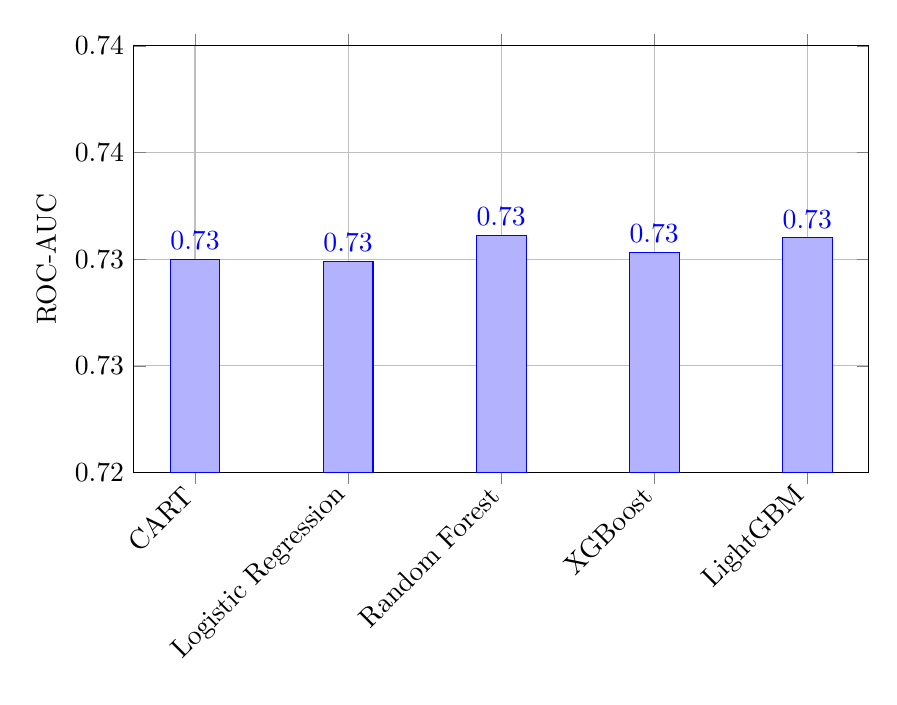
\begin{tikzpicture}
\begin{axis}[
    ybar,
    width=0.9\linewidth,
    height=7cm,
    ylabel={ROC-AUC},
    symbolic x coords={
        CART,
        Logistic Regression,
        Random Forest,
        XGBoost,
        LightGBM
    },
    xtick=data,
    ymin=0.72,
    ymax=0.74,
    nodes near coords,
    nodes near coords align={vertical},
    x tick label style={
        rotate=45,
        anchor=east
    },
    bar width=18pt,
    grid=major
]

\addplot coordinates {
    (CART,0.7300)
    (Logistic Regression,0.7299)
    (Random Forest,0.7311)
    (XGBoost,0.7303)
    (LightGBM,0.7310)
};

\end{axis}
\end{tikzpicture}
\caption{Comparison of predictive model performance using ROC-AUC.}
\label{fig:model_comparison}
\end{figure}

Although Random Forest obtained the highest discrimination score, LightGBM
was selected for the subsequent decision-layer experiments because it
provides competitive predictive performance together with efficient
feature analysis capabilities \cite{ke2017lightgbm}. The objective of the
following stages is not to optimize the prediction model alone, but to
examine how probabilistic outputs can be transformed into operational
risk categories and workflow decisions.

The classification behaviour of the selected model on the held-out test
set is shown in Fig.~\ref{fig:confusion_matrix}.

\begin{figure}[htbp]
\centering
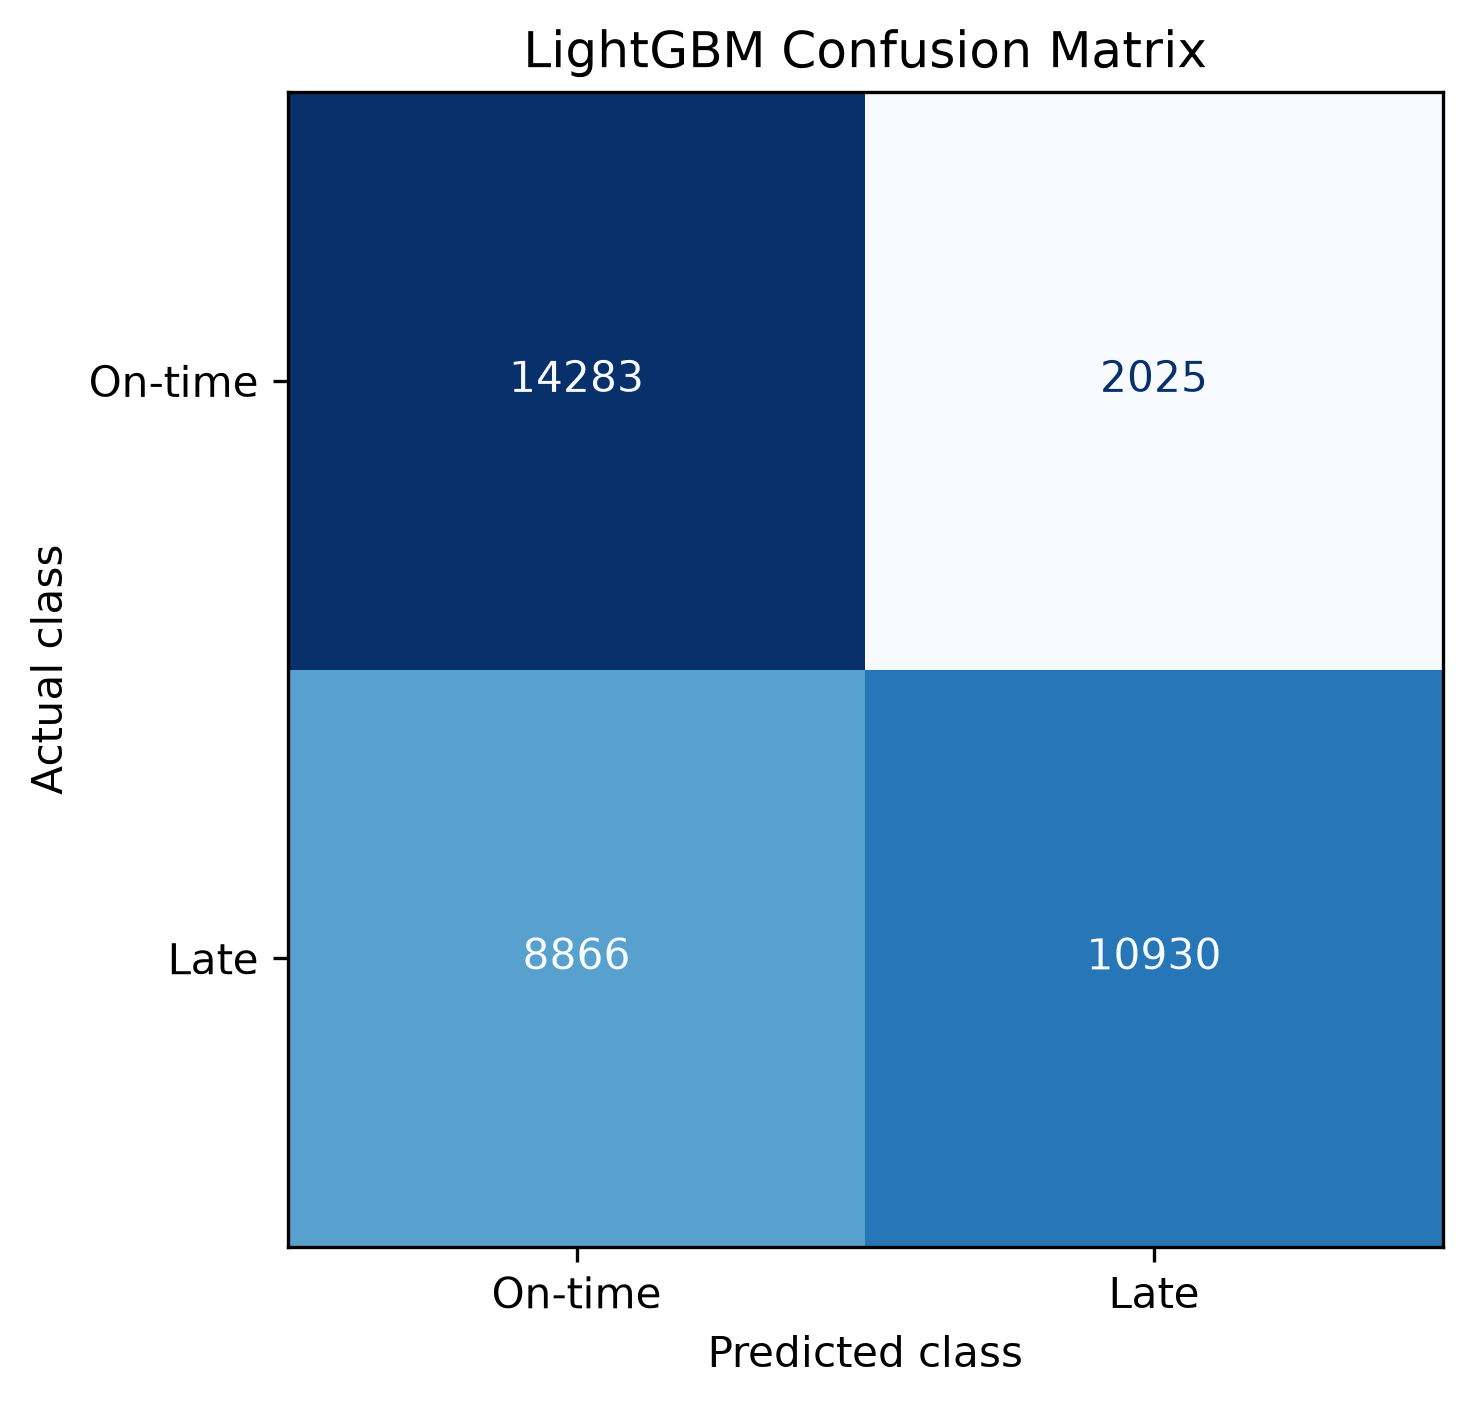
\includegraphics[width=0.65\linewidth]{../../results/confusion_matrix.png}
\caption{Confusion matrix of the selected LightGBM classifier on the held-out test set.}
\label{fig:confusion_matrix}
\end{figure}

The feature importance analysis of the selected model is presented in
Fig.~\ref{fig:feature_importance}. These values indicate the relative
contribution of input variables to the model predictions and are
interpreted as predictive associations rather than causal effects.

\begin{figure}[htbp]
\centering
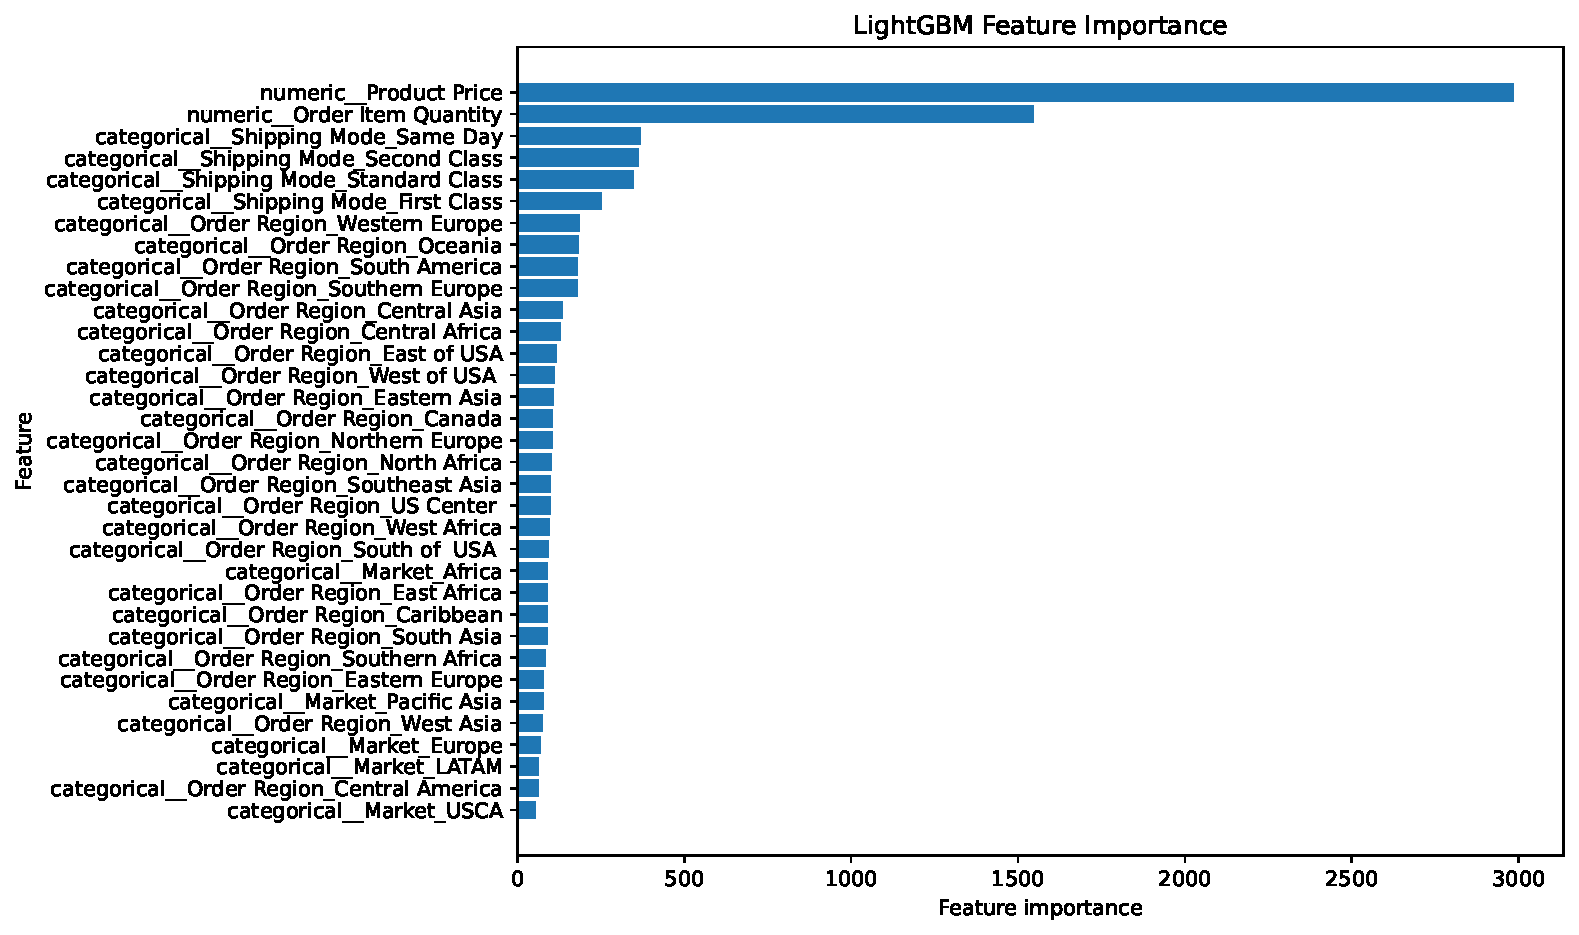
\includegraphics[width=0.85\linewidth]{../../results/feature_importance.pdf}
\caption{Feature importance analysis of the selected LightGBM classifier for late-delivery risk prediction.}
\label{fig:feature_importance}
\end{figure}

\subsection{Risk Stratification}

The probability estimates generated by the selected predictive model
were converted into three operational risk categories:
\texttt{LOW}, \texttt{MEDIUM}, and \texttt{HIGH}. The purpose of this
step is to transform continuous probability outputs into discrete states
that can be used by the subsequent decision layer.

The risk categories were defined using predefined probability thresholds.
Therefore, this analysis evaluates whether the resulting groups exhibit
different historical delivery outcomes rather than optimizing the
thresholds based on the test results.

The observed late-delivery rates within each risk category were:

\begin{equation}
\begin{aligned}
P(Y=1\mid \texttt{LOW}) &= 0.3855,\\
P(Y=1\mid \texttt{MEDIUM}) &= 0.6789,\\
P(Y=1\mid \texttt{HIGH}) &= 0.9320.
\end{aligned}
\end{equation}

The difference between the \texttt{HIGH} and \texttt{LOW} categories
was 0.5465, corresponding to an absolute difference of 54.65 percentage
points in observed late-delivery rate.

The results show an increasing relationship between predicted risk
category and observed late-delivery frequency. The association between
risk category and delivery outcome was statistically significant
($p<0.001$), indicating that the probability-based grouping separates
historical cases according to different levels of observed delivery
risk.

These results support the use of risk categories as an intermediate
decision representation. However, the categories themselves do not
represent automated decisions; operational actions are determined in
the following decision-layer analysis, where economic assumptions and
human-review requirements are considered.

\begin{table}[htbp]
\centering
\caption{Observed late-delivery rates across risk categories.}
\Description{Table showing observed late-delivery rates across LOW, MEDIUM, and HIGH risk categories, including operational interpretations and the percentage point difference between HIGH and LOW levels.}
\label{tab:risk_effectiveness}
\begin{tabular}{lcc}
\hline
Risk Level & Late-Delivery Rate & Operational Interpretation \\
\hline
\texttt{LOW} & 38.55\% & Standard processing \\
\texttt{MEDIUM} & 67.89\% & Additional assessment candidate \\
\texttt{HIGH} & 93.20\% & Priority review candidate \\
\hline
HIGH--LOW Difference & 54.65 percentage points & -- \\
\hline
\end{tabular}
\end{table}

\begin{figure}[htbp]
\centering
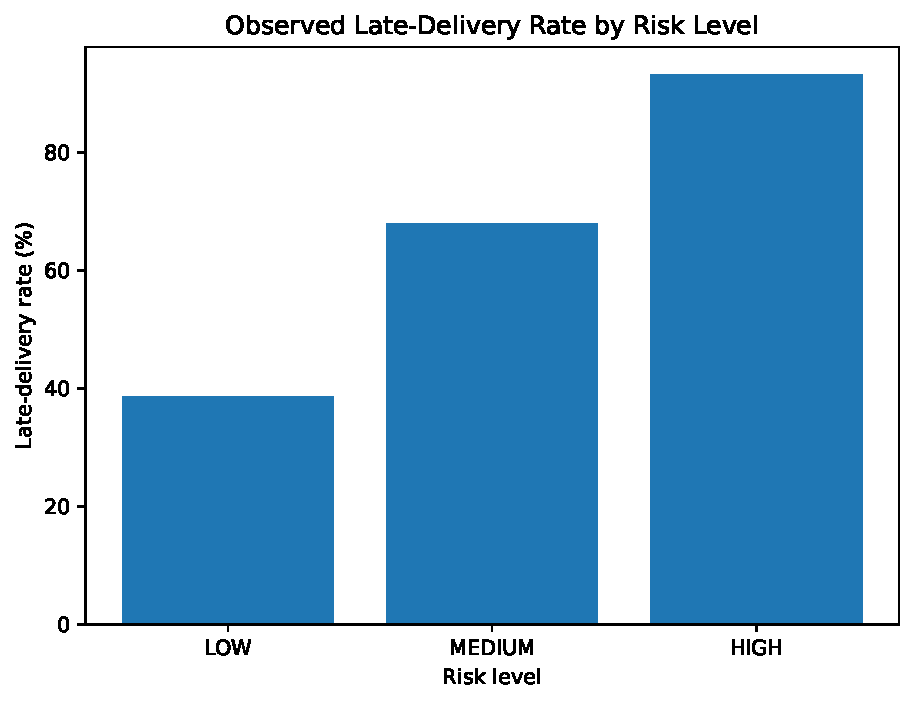
\includegraphics[width=0.85\linewidth]{../../results/risk_effectiveness.pdf}
\caption{Observed late-delivery rates across predefined risk categories.}
\label{fig:risk_effectiveness}
\end{figure}

\subsection{Probability Calibration}

Since the proposed decision layer relies on predicted probabilities as
risk estimates, calibration analysis was performed to examine whether
the predicted probabilities correspond to the observed frequency of
late-delivery events. Unlike discrimination metrics, which evaluate the
ability to rank positive and negative cases, calibration evaluates the
reliability of probability estimates for decision-making purposes
\cite{brier1950verification,niculescu2005predicting,guo2017calibration}.

Two complementary calibration measures were considered: the Brier Score
and Expected Calibration Error (ECE). The Brier Score measures the mean
squared difference between predicted probabilities and observed outcomes
\cite{brier1950verification}, while ECE measures the average difference
between predicted confidence and observed event frequency across
probability intervals \cite{naeini2015obtaining,guo2017calibration}.

The calibration evaluation was performed on the held-out test set
containing 36,104 observations. The selected LightGBM model produced the
following results:

\[
\mathrm{BS}=0.1941,\qquad \mathrm{ECE}=0.0046.
\]

The obtained ECE value indicates that the average deviation between
predicted probabilities and observed frequencies across calibration bins
was limited. The Brier Score provides an additional measure of
probabilistic prediction quality by considering both confidence and
prediction error.

The calibration curve is presented in
Fig.~\ref{fig:calibration_curve}.

\begin{figure}[htbp]
\centering
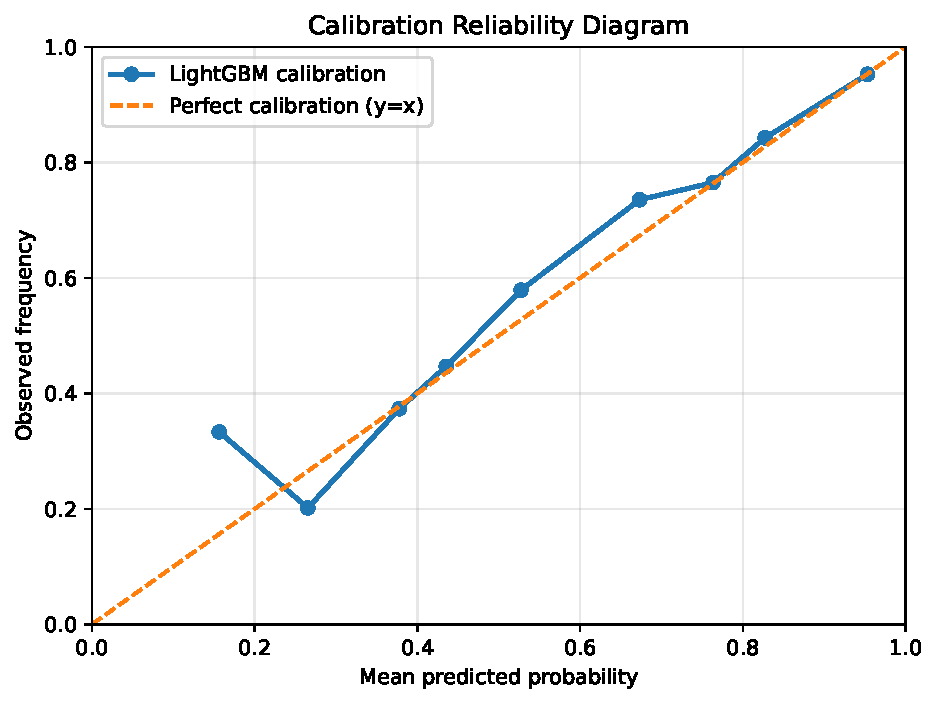
\includegraphics[width=0.8\linewidth]{../../results/calibration_curve.pdf}
\caption{Probability calibration curve of the selected LightGBM model on
the held-out test set.}
\label{fig:calibration_curve}
\end{figure}

The calibration results indicate that the model probabilities provide a
reasonable representation of observed late-delivery frequencies in the
evaluated dataset. This property is important for the subsequent
decision-layer stages, where probability estimates are used for risk
stratification and cost-sensitive evaluation.

\begin{table}[htbp]
\centering
\caption{Probability Calibration Results}
\Description{Table summarizing the probability calibration results, including the Brier Score and Expected Calibration Error for the evaluated model on the test set.}
\label{tab:calibration}
\resizebox{\columnwidth}{!}{
\begin{tabular}{rrrr}
\toprule
Bin & Mean Predicted Probability & Observed Frequency & Absolute Calibration Error \\
\midrule
1 & 0.1564 & 0.3333 & 0.1769 \\
2 & 0.2655 & 0.2017 & 0.0638 \\
3 & 0.3777 & 0.3734 & 0.0043 \\
4 & 0.4354 & 0.4467 & 0.0113 \\
5 & 0.5274 & 0.5789 & 0.0516 \\
6 & 0.6731 & 0.7353 & 0.0622 \\
7 & 0.7634 & 0.7650 & 0.0017 \\
8 & 0.8272 & 0.8424 & 0.0152 \\
9 & 0.9532 & 0.9527 & 0.0005 \\
\bottomrule
\end{tabular}
}
\end{table}


\subsection{SAP-Oriented Decision Layer}

The calibrated probability estimates were transformed into operational
risk states and mapped to SAP-oriented workflow states. The purpose of
this decision layer is to represent the transition between predictive
model outputs and enterprise process decisions, rather than allowing
the prediction model to directly determine operational actions.

The implemented decision mapping was defined as follows:

\[
\texttt{LOW}
\rightarrow
\texttt{SAP\_STANDARD\_PROCESS}
\]

\[
\texttt{MEDIUM}
\rightarrow
\texttt{SAP\_SHIPPING\_PLAN\_REVIEW}
\]

\[
\texttt{HIGH}
\rightarrow
\texttt{SAP\_ORDER\_PRIORITY\_REVIEW}
\]

These workflow states represent logical action categories used in the
simulation environment. They do not correspond to executed SAP
transactions; instead, they provide a structured representation of how
AI-generated risk information could be associated with enterprise
workflow decisions.

The decision layer therefore introduces an intermediate step between
prediction and execution. It converts probabilistic outputs into
interpretable operational states that can be evaluated using additional
criteria, including human review requirements and economic impact.

The SAP-oriented component is implemented as a workflow simulation to
demonstrate the integration pathway between predictive analytics and
enterprise process logic. It is considered a proof-of-concept
representation of the proposed architecture and not a production SAP
deployment.

\subsection{Human-in-the-Loop Decision Control}

Human review was evaluated as a selective control mechanism for cases
that require additional operational assessment. The purpose of this
stage is not to replace the predictive model, but to define when its
recommendation should be subject to human confirmation or intervention
\cite{amershi2019guidelines,shneiderman2020human}.

Among the 36,104 held-out test observations, 12,672 were assigned to
the human-review path, corresponding to a HITL rate of $35.10\%$.

\begin{figure}[htbp]
\centering
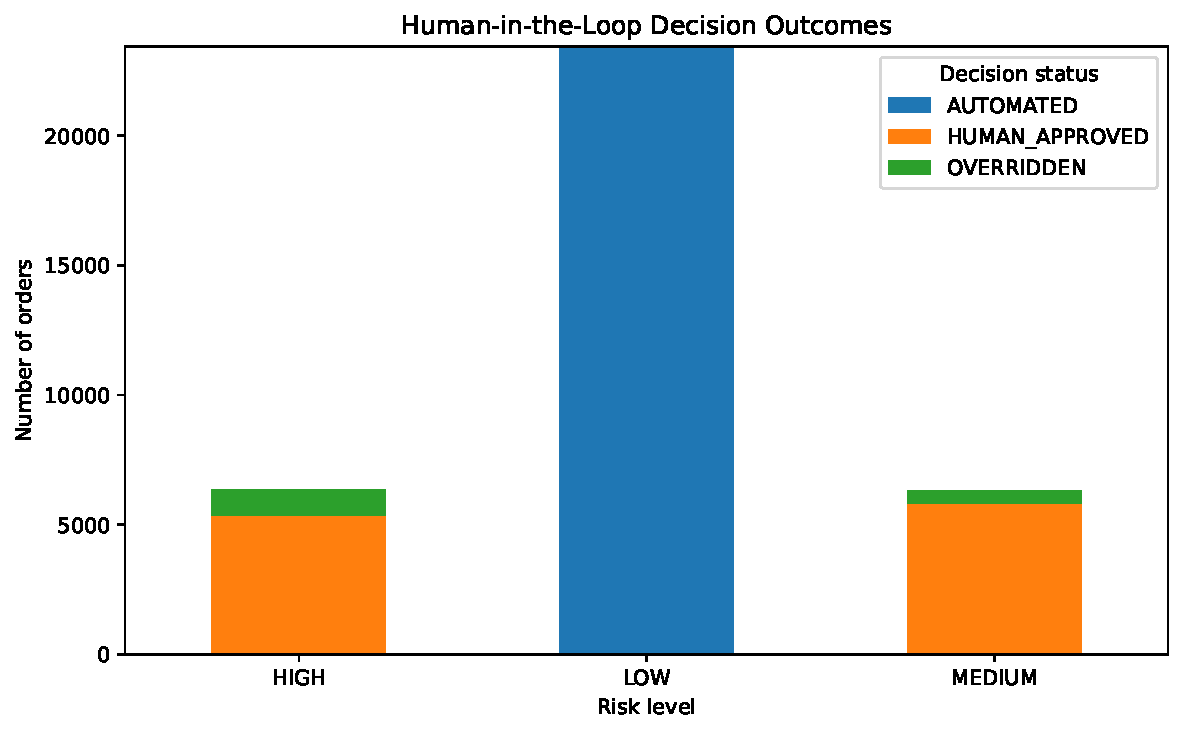
\includegraphics[width=0.85\linewidth]{../../results/human_in_the_loop_flow.pdf}
\caption{Simulated human-review decisions across the operational risk
levels.}
\label{fig:human_in_the_loop}
\end{figure}

The result indicates that human review was required for a subset of
the evaluated cases rather than for every prediction. This provides a
direct measure of the review workload generated by the decision policy.

Representative \texttt{LOW}, \texttt{MEDIUM}, and \texttt{HIGH}-risk
cases were also passed through the simulated workflow to verify that
risk assessment, action selection, human review, and final decision
states were applied consistently. These tests validate the implemented
workflow logic but do not constitute evidence of performance with
actual operational users.

\subsection{Economic Impact and Sensitivity Analysis}

The economic analysis evaluates whether the simulated decision policy
provides a lower expected cost than the baseline policy under the
assumed late-delivery and intervention costs. The analysis is
scenario-based and does not represent observed financial savings.

Under the primary cost configuration, the estimated baseline cost was
$9{,}897{,}690.45$, while the estimated cost after applying the decision
policy was $9{,}561{,}435.12$. The resulting estimated saving was
$336{,}255.34$, corresponding to a saving rate of $3.40\%$.

\begin{table}[htbp]
\centering
\caption{Scenario-based economic evaluation of the decision policy.}
\Description{Table summarizing the scenario-based economic evaluation of the decision policy, listing baseline and decision-policy expected costs, estimated savings, saving rate, and the number of beneficial scenarios.}
\label{tab:economic_impact}
\small
\begin{tabular}{lr}
\toprule
Metric & Value \\
\midrule
Baseline expected cost & 9{,}897{,}690.45 \\
Decision-policy expected cost & 9{,}561{,}435.12 \\
Estimated saving & 336{,}255.34 \\
Estimated saving rate & 3.40\% \\
Beneficial scenarios & 30/49 \\
\bottomrule
\end{tabular}
\end{table}

The result indicates a lower estimated cost under the primary scenario,
but the magnitude of the benefit depends on the assumed cost parameters.
Therefore, a sensitivity analysis was performed using 49 combinations
of late-delivery and intervention costs. The decision policy produced a
positive estimated saving in 30 of the 49 evaluated scenarios.

\begin{figure}[htbp]
\centering
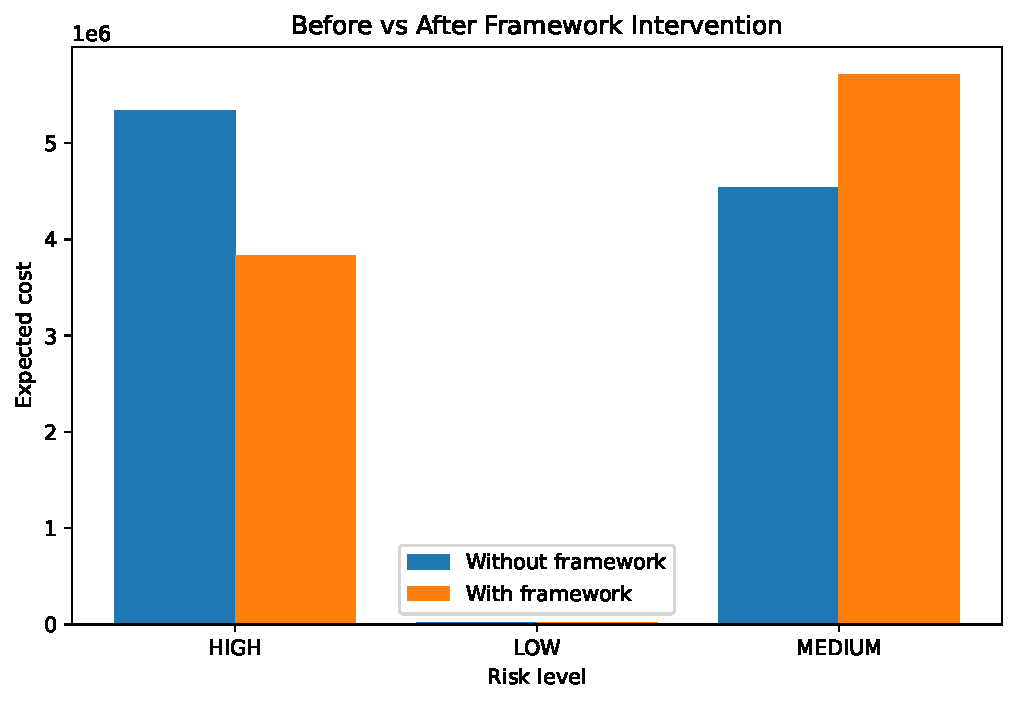
\includegraphics[width=0.85\linewidth]{../../results/before_after_intervention.pdf}
\caption{Estimated baseline and decision-policy costs under the primary
cost scenario.}
\label{fig:before_after}
\end{figure}

The sensitivity results therefore provide a more conservative
interpretation of the economic effect: the decision policy is not
assumed to be beneficial under all cost conditions, but its economic
effect is examined across alternative assumptions.

\subsection{Break-Even Analysis}

Break-even analysis was used to estimate the intervention-cost boundary
under which the decision policy remains economically preferable to the
baseline. The analysis considers the relationship between the assumed
cost of a late-delivery event and the maximum intervention cost that can
be tolerated before the estimated benefit becomes zero.

Seven late-delivery cost levels were evaluated, ranging from \$50 to
\$1,000. Across the evaluated scenarios, the estimated break-even
intervention cost increased as the assumed late-delivery cost increased.

\begin{figure}[htbp]
\centering
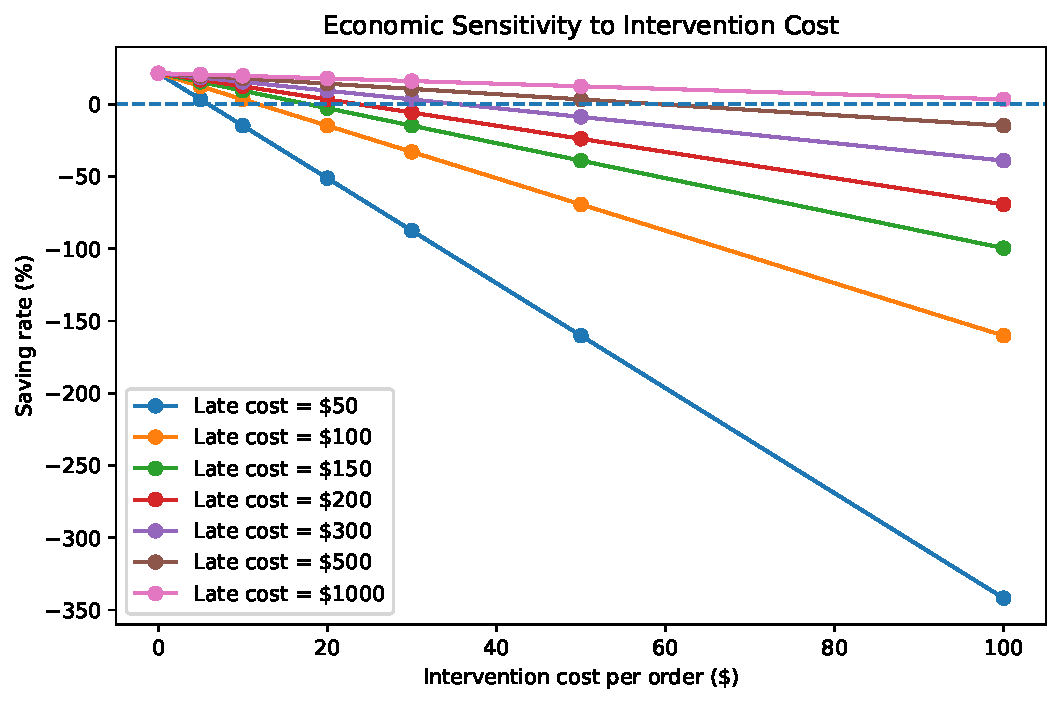
\includegraphics[width=0.85\linewidth]{../../results/cost_sensitivity.pdf}
\caption{Estimated break-even intervention cost under different
late-delivery cost assumptions.}
\label{fig:cost_break_even}
\end{figure}

The result indicates that the economic feasibility of intervention is
sensitive to the relative magnitude of the potential late-delivery loss
and the intervention cost. These values are scenario-based estimates and
should therefore be interpreted as decision thresholds rather than
observed financial outcomes.

\subsection{SAP-Oriented Workflow Validation}

The decision layer was evaluated using representative
\texttt{LOW}, \texttt{MEDIUM}, and \texttt{HIGH}-risk transaction cases.
The test cases were passed through the simulated workflow to verify the
consistent application of risk classification, action selection, human
review requirements, and final decision states.

The generated decision records retained the main attributes produced
during processing, including the predicted probability, risk category,
selected action, workflow state, and human-review status. This provides
a traceable representation of the decision path within the simulation
and supports reproducibility of the evaluated workflow logic.

The validation concerns the implemented workflow simulation and should
not be interpreted as validation of a production SAP integration or of
actual organizational governance processes.

\section{Discussion}

The results provide evidence for a structured transition from
transaction-level prediction to operational decision support. The
predictive models achieved moderate discrimination, with relatively
small differences between the evaluated classifiers. This suggests that
model selection alone does not determine the practical value of the
framework.

The subsequent analyses addressed the stages that follow prediction.
Calibrated probabilities were used to construct three risk categories,
and the observed late-delivery rates increased from the LOW to the HIGH
category. This provides empirical support for using the model output as
an input to risk-based decision rules rather than treating the prediction
as a final decision.

The economic analysis further showed that the usefulness of an
intervention depends on its assumed costs. The primary scenario produced
an estimated saving, while the sensitivity analysis showed that positive
benefit was not obtained under all evaluated cost configurations. The
break-even analysis therefore provides an additional decision boundary
for determining when an intervention may no longer be economically
justified.

Human review was implemented as a selective control step. The
simulation generated a measurable review workload rather than assuming
that every prediction requires human intervention. The SAP-oriented
workflow simulation then represented how the resulting risk state,
action, review status, and final decision could be organized within an
enterprise workflow.

Taken together, these results address the research problem at the level
supported by the study: they demonstrate a simulated pathway for
transforming logistics predictions into risk-based decisions, economic
assessments, human-review states, and SAP-oriented workflow records.
The study does not establish the effectiveness of a production SAP
integration or of human decision-making with real operational users.
\section{Conclusion}

This paper demonstrated a simulated framework for translating predictive logistics analytics into structured, risk-based operational decisions within enterprise systems. By integrating machine learning classification, probability calibration, economic sensitivity analysis, and selective human review into an SAP-oriented workflow simulation, the study established a traceable pathway from transaction-level prediction to operational execution. All source code, simulation scripts, and data processing pipelines used to generate the results and figures in this study are publicly available for reproducibility at \url{https://github.com/majdkassem/ICIES_2026_Explainable_AI_SAP}. Future work will focus on validating these components within live production environments and evaluating human-in-the-loop decision-making dynamics with real operational users.

\bibliographystyle{ACM-Reference-Format}
\bibliography{references}

\end{document}